\chapter{Algoritmi Geometrici}
\label{Geom_Algos}
%
\section{Introduzione}
La geometria computazionale è la branca dell'Informatica che studia le strutture dati e gli algoritmi efficienti per la soluzione di problemi di natura geometrica e la loro implementazione al calcolatore. Storicamente, è considerato uno dei campi più antichi del calcolo, anche se la geometria computazionale moderna è uno sviluppo recente. La ragione principale per lo sviluppo della geometria computazionale è stata dovuta ai progressi compiuti nella computer grafica, \ac{CAD}, \ac{CAM} e nella visualizzazione matematica. Ad oggi, le applicazioni della geometria computazionale si trovano nella robotica, nella progettazione di circuiti integrati, nella visione artificiale, in \ac{CAE} e nel \ac{GIS}.\\
I rami principali della geometria computazionale sono:
\begin{itemize}
	\item \textit{Calcolo combinatorio} (o \textit{geometria algoritmica}), che si occupa di oggetti geometrici come entità discrete. Ad esempio, può essere utilizzato per determinare il poliedro o il poligono più piccolo che contiene tutti i punti forniti, o più formalmente, dato un insieme di punti, si deve determinare il più piccolo insieme convesso che li contenga tutti (problema dell'inviluppo convesso).
	\item \textit{Geometria di calcolo} numerica (o \ac{CAGD}), che si occupa principalmente di rappresentare oggetti del mondo reale in forme adatte per i calcoli informatici nei sistemi \ac{CAD} e \ac{CAM}. Questo ramo può essere visto come uno sviluppo della geometria descrittiva ed è spesso considerato un ramo della computer grafica o del \ac{CAD}. Entità importanti di questo ramo sono superfici e curve parametriche, come ad esempio le \textit{spline} e \textit{curve di Bézier}.
\end{itemize}
In questo capitolo tutti gli algoritmi che verranno utilizzati in seguito durante l'analisi geometrica dell'intersezione tra pneumatico e superfice stradale saranno trattati. Questi algoritmi sono la soluzione di alcuni semplici ma molto importanti problemi, che devono essere risolti in modo efficiente. In particolare le intersezioni tra:
\begin{itemize}
	\item punto e segmento (sul piano);
	\item punto e circonferenza (sul piano);
	\item raggio e circonferenza (sul piano);
	\item raggio e triangolo (sullo spazio);
\end{itemize}
saranno esaminato al fine di trovare la massima prestazione in termini di \textit{efficienza computazionale}.
%
\section{Point-Segment Intersection}

%
\section{Point-Circle Intersection}
Having a circle with center $C = (x_c, y_c)$ and radius $r$, the problem consists in finding out whether a query point $P = (x_p, y_p)$ is inside, outside or on the circle.
%
\begin{figure}
	\centering
	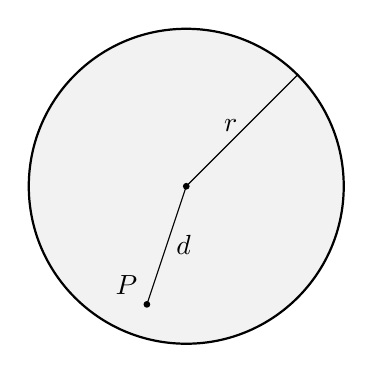
\begin{tikzpicture}
	\def\r{2};
	\coordinate (C) at (0,0) node[above left] {$C$};
	\draw[thick, fill=gray!10](C) circle (\r);
	\coordinate (P) at (-0.5,-1.5);
	\draw[fill] (C) circle [radius=1pt];
	\draw[fill] (P) circle [radius=1pt];
	\draw(C) -- (P)  node[above left] {$P$} node[pos=0.5, right] {$d$};
	\draw(C) -- ({sqrt(\r)},{sqrt(\r)}) node[pos=0.4, above] {$r$};
	\end{tikzpicture}
	\caption{Point-circle intersection problem scheme.}
\end{figure}
%
The solution to the problem is simple: the distance between the circle center $C$ and the query point $P$ is given by the \textit{Pythagorean theorem} as
\begin{equation}
	d=\sqrt{(x_p-x_c)^2 + (y_p-y_c)^2}
\end{equation}
The query point $P$ is \textit{inside} the circle if $d<r$, on the circle if $d = r$, and \textit{outside} the circle if $d > r$. Little work can be saved by comparing $d^2$ with $r^2$ instead: the point $P$ is \textit{inside} the circle if $d^2<r^2$, on the circle if $d^2 = r^2$, and \textit{outside} the circle if $d^2 > r^2$. Thus, the final comparison will be between the number $(x_p-x_c)^2 + (y_p-y_c)^2$ and $r^2$.\\
The \textit{inputs} of the point-circle intersection algorithm are:
\begin{itemize}
	\item the circle center $C = (x_c, y_c)$;
	\item the circle radius $r$;
	\item a query point $P=(x_p, y_p)$.
\end{itemize}
The \textit{output} could be an integer which value is:
\begin{itemize}
	\item 0 if the point is outside;
	\item 1 if the point is inside;
	\item 2 if the point is on the circle.
\end{itemize}
Another option could be a boolean which value is:
\begin{itemize}
	\item false if the point is outside;
	\item true if the point is inside or on the circle.
\end{itemize}
%
\begin{figure}
\hfill
	\begin{subfigure}{.45\textwidth}
	\centering
	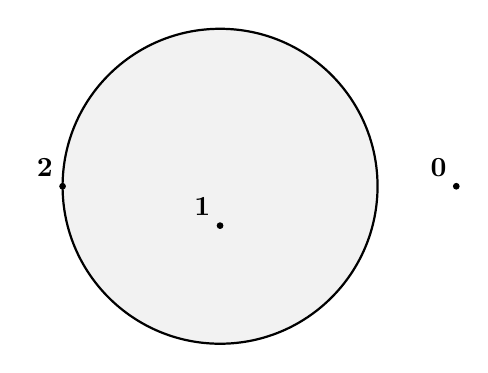
\begin{tikzpicture}
	\def\r{2};
	\coordinate (C) at (0,0);
	\draw[thick, fill=gray!10](C) circle (\r);
	\draw[fill] (0,-0.5) circle [radius=1pt] node[above left] {$\mathbf{1}$};
	\draw[fill] (-\r,0) circle [radius=1pt] node[above left] {$\mathbf{2}$};
	\draw[fill] (3,0) circle [radius=1pt] node[above left] {$\mathbf{0}$};
	\end{tikzpicture}
	\caption{Integer output}
	\end{subfigure}
\hfill
\begin{subfigure}{.45\textwidth}
	\centering
	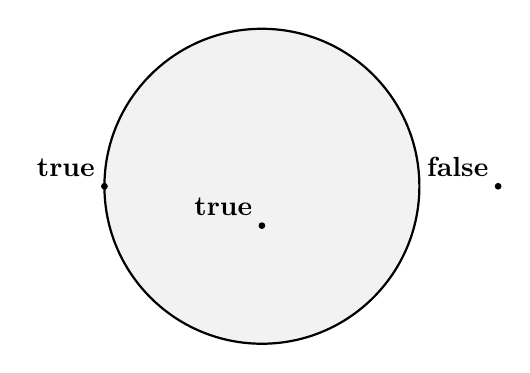
\begin{tikzpicture}
	\def\r{2};
	\coordinate (C) at (0,0);
	\draw[thick, fill=gray!10](C) circle (\r);
	\draw[fill] (0,-0.5) circle [radius=1pt] node[above left] {$\mathbf{true}$};
	\draw[fill] (-\r,0) circle [radius=1pt] node[above left] {$\mathbf{true}$};
	\draw[fill] (3,0) circle [radius=1pt] node[above left] {$\mathbf{false}$};
	\end{tikzpicture}
	\caption{Boolean output}
\end{subfigure}
\hfill
\caption{Output schemes of the point-circle intersection problem.}
\end{figure}
On \figurename{ \ref{Pointcircle}} the schemes for the point-circle intersection algorithm with integer and boolean outputs are reported.\\
%
\begin{figure}[htbp]
\hfill
	\begin{subfigure}[t]{.4\linewidth}
		\raggedright
		\textit{With integer output}\\
		\vspace{.5em}
		$d = (x_p-x_c)^2 + (y_p-y_c)^2$\\
		$\mathbf{if} \, (d > r^2) \{$\\
		\quad $\mathbf{return \, 0}$\\
		$\} \, \mathbf{else \, if} \, (d < r^2) \{$\\
		\quad $\mathbf{return \, 1}$\\
		$\} \, \mathbf{else} \, \{$\\
		\quad $\slash\slash \, d = r^2$\\
		\quad $\mathbf{return \, 2}$\\
		$\}$\\
	\end{subfigure}
\hfill
	\begin{subfigure}[t]{.4\textwidth}
		\raggedright
		\textit{With boolean output}\\
		\vspace{.5em}
		$d = (x_p-x_c)^2 + (y_p-y_c)^2$\\
		$\mathbf{if} \, (d > r^2) \{$\\
		\quad $\mathbf{return \, false}$\\
		$\} \, \mathbf{else} \, \{$\\
		\quad $\slash\slash \, d <= r^2$\\
		\quad $\mathbf{return \, true}$\\
		$\}$\\		
	\end{subfigure}
\hfill
\caption{Point-circle intersection algorithm schemes.}
\label{Pointcircle}
\end{figure}
%
\section{Ray-Circle Intersection}

%
\section{Ray-Triangle Intersection}
Having a triangle with vertices $(V_1,V_2,V_3)$ and a ray $R$ with origin $R_O$ and direction $R_D$, the problem consists in finding out whether the ray hits or not the triangle and if so, where is the intersection point $P$.
%
\begin{figure}[htbp]
	\centering
	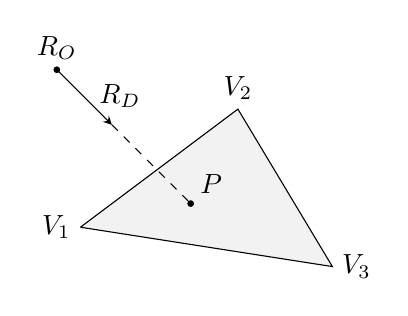
\begin{tikzpicture}
	\coordinate [label=left:$V_1$] (A) at (-1,-0.5);
	\coordinate [label=above:$V_2$] (B) at (1,1);
	\coordinate [label=right:$V_3$] (C) at (2.2,-1);
	\draw[fill=gray!10] (A) -- (B) -- (C) -- (A);
	\def\xp{0.4};
	\def\yp{-0.2};
	\def\xd{-1};
	\def\yd{1};
	\def\mag{1.7};
	\coordinate [label=above right:$P$] (P) at (\xp,\yp);
	\coordinate [label={[shift={(0.1,0.1)}]$R_D$}] (RD) at (\xp+\xd,\yp+\yd);
	\coordinate [label=above:$R_O$] (RO) at (\xp+\xd*\mag,\yp+\yd*\mag);
	\draw[fill] (P) circle [radius=1pt];
	\draw[fill] (RO) circle [radius=1pt];
	\draw[-stealth] (RO) -- (RD);
	\draw[dashed] (RD) -- (P);
	\end{tikzpicture}
	\caption{Ray-triangle intersection problem scheme.}
\end{figure}
%
Over the last decades, plenty of algorithms for solving this problem had been purposed, so there are several solutions to the ray/triangle or ray-triangle intersection problem. Three of the most relevant algorithms are:
\begin{itemize}
	\item \textit{Badouel} algorithm;
	\item \textit{Segura} algorithm;
	\item \textit{M\"oller-Trumbore} algorithm.
\end{itemize}
As \citeauthor{RayTriangle} states in \cite{RayTriangle}, the M\"oller-Trumbore's is the faster algorithm when the normal and/or the projection plane have not been previously stored, as in this thesis.\\
%
\subsection{M\"oller-Trumbore Algorithm}

\begin{figure}[htbp]
	\centering
	\hfill
	\begin{subfigure}[t]{.3\linewidth}
		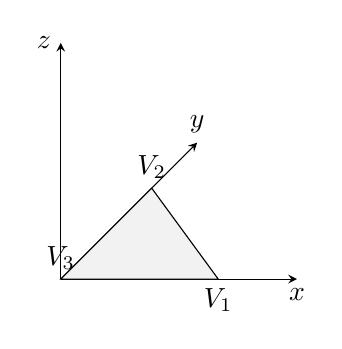
\begin{tikzpicture}
			\coordinate (O) at (0,0,0);
			\def\axisl{3}
			\draw[-stealth] (O) -- (\axisl,0,0) node[below]{$x$};
			\draw[-stealth] (O) -- ({sqrt(\axisl)},{sqrt(\axisl)},0) node[above]{$y$};
			\draw[-stealth] (O) -- (0,\axisl,0) node[left]{$z$};
			
			\coordinate [label=below:$V_1$] (V1) at ({\axisl/1.5},0,0);
\coordinate [label=above:$V_2$] (V2) at ({sqrt(\axisl)/1.5},{sqrt(\axisl)/1.5},0);
\coordinate [label=above:$V_3$] (V3) at (0,0,0);
			
			\draw[fill=gray!10] (V1) -- (V2) -- (V3) -- (V1);

		\end{tikzpicture}
	\end{subfigure}
\hfill
\begin{subfigure}[t]{.3\linewidth}
	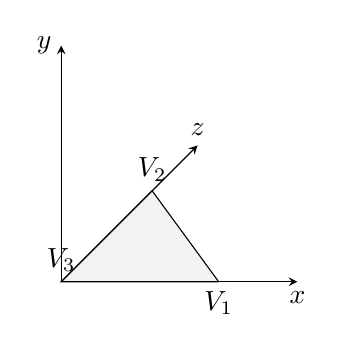
\begin{tikzpicture}
			\coordinate (O) at (0,0,0);
			\def\axisl{3}
		\draw[-stealth] (O) -- (\axisl,0,0) node[below]{$x$};
\draw[-stealth] (O) -- ({sqrt(\axisl)},{sqrt(\axisl)},0) node[above]{$z$};
\draw[-stealth] (O) -- (0,\axisl,0) node[left]{$y$};
			
			\coordinate [label=below:$V_1$] (V1) at ({\axisl/1.5},0,0);
			\coordinate [label=above:$V_2$] (V2) at ({sqrt(\axisl)/1.5},{sqrt(\axisl)/1.5},0);
			\coordinate [label=above:$V_3$] (V3) at (0,0,0);
			

			
			\draw[fill=gray!10] (V1) -- (V2) -- (V3) -- (V1);

	\end{tikzpicture}
\end{subfigure}
\hfill
\begin{subfigure}[t]{.3\linewidth}
	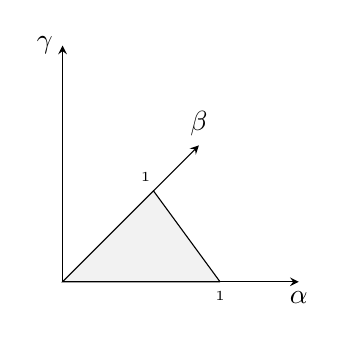
\begin{tikzpicture}
		\coordinate (O) at (0,0,0);
		\def\axisl{3}
		\draw[-stealth] (O) -- (\axisl,0,0) node[below]{$\alpha$};
		\draw[-stealth] (O) -- ({sqrt(\axisl)},{sqrt(\axisl)},0) node[above]{$\beta$};
		\draw[-stealth] (O) -- (0,\axisl,0) node[left]{$\gamma$};
		
		\coordinate [label={[below,font=\tiny]:$1$}] (V1) at ({\axisl/1.5},0,0);
		\coordinate [label={[shift={(-0.1,0.0)},font=\tiny]:$1$}] (V2) at ({sqrt(\axisl)/1.5},{sqrt(\axisl)/1.5},0);
		\coordinate (V3) at (0,0,0);
		
		\draw[fill=gray!10] (V1) -- (V2) -- (V3) -- (V1);
	\end{tikzpicture}
\end{subfigure}
\hfill
\caption{Transformation and base change of ray in M\"oller-Trumbore algorithm.}
\end{figure}



The inputs of the M\"oller-Trumbore algorithm are:
\begin{itemize}
	\item Triangle vertices $(V_1, V_2, V_3)$;
	\item Segment points $(Q_1, Q_2)$.
\end{itemize}
%
\begin{figure}[htbp]
\hfill
	\begin{subfigure}[t]{.4\linewidth}
		\raggedright
		\textit{With back-face culling}\\
		\vspace{.5em}
		$Q = Q_2 - Q_1$\\
		$E_1 = V_2 - V_1$\\
		$E_2 = V_3 - V_1$\\
		$A = Q \times E_2$\\
		$D = A \cdot E_1$\\
		$\mathbf{if} \, (D > \varepsilon) \{$\\
		\quad $T = Q_1 - V_1$\\
		\quad $u = A \cdot T$\\
		\quad $\mathbf{if} \, (u < 0.0 \, || \, u > D) \{$\\
		\quad \quad $\mathbf{return \, false}$\\
		\quad $\}$\\
		\quad $B = T \times E_1$\\
		\quad $v = B \cdot Q$\\
		\quad $\mathbf{if} \, (v < 0.0 \, || \, u + v > D) \{$\\
		\quad \quad $\mathbf{return \, false}$\\
		\quad $\}$\\
		$\} \, \mathbf{else \, if} \, (D < -\varepsilon) \{$\\
		\quad $T = Q_1 - V_1$\\
		\quad $u = A \cdot T$\\
		\quad $\mathbf{if} \, (u > 0.0 \, || \, u < D) \{$\\
		\quad \quad $\mathbf{return \, false}$\\
		\quad $\}$\\
		\quad $B = T \times E_1$\\
		\quad $v = B \cdot Q$\\
		\quad $\mathbf{if} \, (v > 0.0 \, || \, u + v < D) \{$\\
		\quad \quad $\mathbf{return \, false}$\\
		\quad $\}$\\
		$\} \, \mathbf{else} \, \{$\\
		\quad $\mathbf{return \, false}$\\
		$\}$\\
		$D_{inv} = 1.0 / D$\\
		$t = (B \cdot E_2) * D_{inv}$\\
		$\mathbf{if} \, (t > 0.0) \{$\\
		\quad $P = Q + D * t$\\
		\quad $\mathbf{return \, true}$\\
		$\} \, \mathbf{else} \, \{$\\
		\quad $\mathbf{return \, false}$\\
		$\}$\\
	\end{subfigure}
\hfill
	\begin{subfigure}[t]{.4\textwidth}
		\raggedright
		\textit{Without back-face culling}\\
		\vspace{.5em}
		$Q = Q_2 - Q_1$\\
		$E_1 = V_2 - V_1$\\
		$E_2 = V_3 - V_1$\\
		$A = Q \times E_2$\\
		$D = A \cdot E_1$\\
		$\mathbf{if} \, (D < \varepsilon) \{$\\
		\quad $\mathbf{return \, false}$\\
		$\}$\\
		$T = Q_1 - V_1$\\
		$u = A \cdot T$\\
		$\mathbf{if} \, (u < 0.0 \, || \, u > D) \{$\\
		\quad $\mathbf{return \, false}$\\
		$\}$\\
		$B = T \times E_1$\\
		$v = B \cdot Q$\\
		$\mathbf{if} \, (v < 0.0 \, || \, u + v > D) \{$\\
		\quad \quad $\mathbf{return \, false}$\\
		$\}$\\
		$D_{inv} = 1.0 / D$\\
		$t = (B \cdot E_2) * D_{inv}$\\
		$\mathbf{if} \, (t > 0.0) \{$\\
		\quad $P = Q + D * t$\\
		\quad $\mathbf{return \, true}$\\
		$\} \, \mathbf{else} \, \{$\\
		\quad $\mathbf{return \, false}$\\
		$\}$\\
	\end{subfigure}
\hfill
\caption{Ray-triangle intersection algorithm schemes.}
\end{figure}